\chapter{Numerical Solution of Adjoint Equations}
\label{chapter-four}

This section details the derivation of the adjoint equations to be solved in
conjuction with the primal flow equations.  The primary goal of this research is
to compute sensitivities of aerodynamic and aerothermodynamic quantities to
design variables.  To achieve this, the sensitivity to the primal flow equation
formulation must first be solved.  For a discrete adjoint formulation, this
requires a solution of costate variables, relating a change in the flow equation
residual to a change in the function of interest.  Because of the large number
of equations required in a reacting gas solver, the adjoint solver will suffer
from the quadratic scaling in computational cost and memory required similarly
to the primal flow solver.  To mitigate this, a decoupled scheme is derived that
is consistent with the decoupled flow solver.

\section{Discrete Adjoint Derivation}

The derivation for the discrete adjoint begins with forming the Lagrangian as
%------------------------------------------------------------------------------%
\begin{equation}
  L(\md,\mq,\mx,\mathbf{\Lambda})=f(\md,\mq,\mx)
  +\mathbf{\Lambda}^T\mr(\md,\mq,\mx)
\end{equation}
%------------------------------------------------------------------------------%
Where $\mr$ is the residual of the flow equations.  Differentiating with respect
to the design variables $\md$ yields
%------------------------------------------------------------------------------%
\begin{equation}
  \pd{L}{\md} = 
  \Bigg\{\pd{f}{\md}+\bigg[\pd{\mx}{\md}\bigg]^T \pd{f}{\mx}\Bigg\} 
  + \bigg[\pd{\mq}{\md}\bigg]^T
  \Bigg\{\pd{f}{\mq}+\bigg[\pd{\mr}{\mq}\bigg]^T \mathbf{\Lambda}\Bigg\}
  +\Bigg\{\bigg[\pd{\mr}{\md}\bigg]^T
  +\bigg[\pd{\mx}{\md}\bigg]^T\bigg[\pd{\mr}{\mx}\bigg]^T\Bigg\}\mathbf{\Lambda}
  \label{dL}
\end{equation}
%------------------------------------------------------------------------------%
To eliminate the dependence of conserved variables $\mq$ on the design
variables, we solve the adjoint equation
%------------------------------------------------------------------------------%
\begin{equation}
  \bigg[\pd{\mr}{\mq}\bigg]^T\mathbf{\Lambda} = -\pd{f}{\mq}
  \label{adjoint-main}
\end{equation}
%------------------------------------------------------------------------------%
Where the Lagrange multipliers (also known as costate variables),
$\mathbf{\Lambda}$ are the cost function dependence on the residual
%------------------------------------------------------------------------------%
\begin{equation}
  \mathbf{\Lambda}=-\pd{f}{\mr}
\end{equation}
%------------------------------------------------------------------------------%
This can ultimately be used in error estimation and sensitivity analysis for
design optimization.  With the second term in eq.~(\ref{dL}) eliminated, the
derivative of the Lagrangian becomes
%------------------------------------------------------------------------------%
\begin{equation}
  \pd{L}{\md}=
  \Bigg\{\pd{f}{\md}+\bigg[\pd{\mx}{\md}\bigg]^T \pd{f}{\mx}\Bigg\}
  +\Bigg\{\bigg[\pd{\mr}{\md}\bigg]^T
  +\bigg[\pd{\mx}{\md}\bigg]^T\bigg[\pd{\mr}{\mx}\bigg]^T\Bigg\}\mathbf{\Lambda}
  \label{obj-function}
\end{equation}
%------------------------------------------------------------------------------%
By solving the adjoint equation in \eref{adjoint-main}) to obtain the costate
variable vector, $\mathbf{\Lambda}$, we can now use a non-linear optimizer to
determine the optimum set of design variables, $\md^*$. This can be done using
{\bf SNOPT\cite{snopt-manual}}, {\bf KSOPT\cite{KSOPT}}, or {\bf
  NPSOL\cite{npsol-manual}} in FUN3D, as well as a host of other non-linear
  optimizers.

\section{Block Jacobi Adjoint Decoupling}

It is possible to decoupled the adjoint equations in a fashion similiar to that
done to the primal flow equations.  In this decoupled adjoint formulation, the
conserved variables are split identically to flow equations, with the
fully-coupled vector of conserved variables
%------------------------------------------------------------------------------%
\begin{equation}
	\vU =
  \begin{pmatrix}
 		\rho_1    \\
		\vdots    \\
		\rho_{ns} \\
    \rho \vu  \\
		\rho E    \\
	\end{pmatrix}
  \label{all-vars}
 \end{equation}
%------------------------------------------------------------------------------%
 split into
%------------------------------------------------------------------------------%
\begin{equation}
	\begin{matrix}
		\mathbf{U}'=\begin{pmatrix}
			\rho \\
			\rho \vu \\
			\rho E
		\end{pmatrix},\quad &
		\mathbf{\hat{U}}=\begin{pmatrix}
			\rho_1 \\
			\vdots \\
			\rho_{ns}
		\end{pmatrix}
	\end{matrix}
  \label{dc-vars}
\end{equation}
%------------------------------------------------------------------------------%
With this splitting, the mixture equations for single point in the global system
of the decoupled flow solve can be written as
%------------------------------------------------------------------------------%
\begin{equation}
  \frac{V}{\Delta t}\mi + 
  \begin{pmatrix}
    \rdiff{\rho}{\rho} & \rdiff{\rho}{\rho \vu} & \rdiff{\rho}{\rho E} \\ \\
    \rdiff{\rho \vu}{\rho} & \rdiff{\rho \vu}{\rho \vu} & \rdiff{\rho \vu}{\rho E} \\ \\
    \rdiff{\rho E}{\rho} & \rdiff{\rho E}{\rho \vu} & \rdiff{\rho E}{\rho E}
  \end{pmatrix}
  \begin{pmatrix}
    \Delta \rho \\ \\
    \Delta \rho \vu \\ \\
    \Delta \rho E
  \end{pmatrix}
  =
  \begin{pmatrix}
    \res{\rho} \\ \\
    \res{\rho \vu} \\ \\
    \res{\rho E}
  \end{pmatrix}
  \label{approx-jac}
\end{equation}
%------------------------------------------------------------------------------%
Likewise, the species mass equations for a single point can be written as
%------------------------------------------------------------------------------%
\begin{equation}
  \frac{V}{\Delta t}\mi + 
  \begin{pmatrix}
    \rdiff{\rho_1}{c_1} & \cdots & \rdiff{\rho_{1}}{c_{ns}} \\ \\
    \vdots & \ddots & \vdots \\ \\
    \rdiff{\rho_{ns}}{c_1} & \cdots & \rdiff{\rho_{ns}}{c_{ns}}
  \end{pmatrix}
  \begin{pmatrix}
    \Delta c_1 \\ \\
    \vdots \\ \\
    \Delta c_{ns}
  \end{pmatrix}
  =
  \begin{pmatrix}
    \res{\rho_1} \\ \\
    \vdots \\ \\
    \res{\rho_{ns}}
  \end{pmatrix}
  \label{approx-jac-dc}
\end{equation}
%------------------------------------------------------------------------------%
Examining \erefs{approx-jac}{approx-jac-dc} shows that there are clearly some
physical dependencies being omitted, namely $\rdiff{\rho_s}{\rho}$,
$\rdiff{\rho}{c_s}$, $\rdiff{\rho \vu}{c_s}$, and $\rdiff{\rho E}{c_s}$.  It has
been found\cite{candler} that omitting this dependencies does not hinder convergence
the primal flow solver; however, because the adjoint requires an exact
linearization of the converged steady-state solution, these must be accounted
for in the decoupled adjoint formulation.

The next step is to reconcile the split conserved variables, $\mathbf{U}'$ and
$\mathbf{\hat{U}}$, with the conserved variable vector $\mq$ in the discrete
adjoint formulation given in \eref{adjoint-main}. The most intuitive and
staightforward way to do this is to forgo solving for the species mass $\rho_s$
in lieu of the species mass fraction $c_s$.  Thus, $\mq$ can be expressed as
%------------------------------------------------------------------------------%
\begin{equation}
  \mq =
  \begin{pmatrix}
  	\rho \\
  	\rho u \\
  	\rho v \\
  	\rho w \\
  	\rho E \\
    c_1 \\
    \vdots \\
    c_{ns}
  \end{pmatrix}
  \label{q-vec}
\end{equation}
%------------------------------------------------------------------------------%
This allows the linearizations in \erefs{approx-jac}{approx-jac-dc} to be used
in the adjoint formulation, by augmenting them with the previously omitted
linearizations.  Replacing $\rdiff{}{\mq}$ with the fully-coupled system, the
adjoint system becomes
%------------------------------------------------------------------------------%
\begin{equation}
  \begin{pmatrix}
    \rtdiff{\rho}{\rho} & \rtdiff{\rho \vu}{\rho} & 
    \rtdiff{\rho E}{\rho} & \rtdiff{\rho_s}{\rho} \\ \\
    \rtdiff{\rho}{\rho \vu} & \rtdiff{\rho \vu}{\rho \vu} & 
    \rtdiff{\rho E}{\rho \vu} & \rtdiff{\rho_s}{\rho \vu} \\ \\
    \rtdiff{\rho}{\rho E} & \rtdiff{\rho \vu}{\rho E} & 
    \rtdiff{\rho E}{\rho E} & \rtdiff{\rho_s}{\rho E} \\ \\
    \rtdiff{\rho}{c_s} & \rtdiff{\rho \vu}{c_s} & 
    \rtdiff{\rho E}{c_s} & \rtdiff{\rho_s}{c_s}
  \end{pmatrix}
  \begin{pmatrix}
    \adjlam{\rho} \\ \\
    \adjlam{\rho \vu} \\ \\
    \adjlam{\rho E} \\ \\
    \adjlam{c_s}
  \end{pmatrix}
  = -
  \begin{pmatrix}
    \pd{f}{\rho} \\ \\
    \pd{f}{\rho \vu} \\ \\
    \pd{f}{\rho E} \\ \\
    \pd{f}{c_s}
  \end{pmatrix}
  \label{full-adjoint}
\end{equation}
%------------------------------------------------------------------------------%
Thus the jacobian in \eref{full-adjoint} is the completed one of
\erefs{approx-jac}{approx-jac-dc}.  While this is useful, the advantage of
decoupling the species equations from the mixture equations was to speed up the
linear solver and save memory.  Solving \eref{full-adjoint} is roughly
equivalent to solving the fully-coupled system of equations, which undermines
both of these goals; so, an alternative solution strategy must be formulated.  If
a block jacobi scheme is employed, the system can be decoupled once again as
%------------------------------------------------------------------------------%
\begin{equation}
  \begin{pmatrix}
    \rtdiff{\rho}{\rho}     & \rtdiff{\rho \vu}{\rho}     & \rtdiff{\rho E}{\rho} \\ \\
    \rtdiff{\rho}{\rho \vu} & \rtdiff{\rho \vu}{\rho \vu} & \rtdiff{\rho E}{\rho \vu} \\ \\
    \rtdiff{\rho}{\rho E}   & \rtdiff{\rho \vu}{\rho E}   & \rtdiff{\rho E}{\rho E}
  \end{pmatrix}
  \begin{pmatrix}
    \adjlam{\rho} \\ \\
    \adjlam{\rho \vu} \\ \\
    \adjlam{\rho E}
  \end{pmatrix}
  = -
  \begin{pmatrix}
    \pd{f}{\rho} \\ \\
    \pd{f}{\rho \vu} \\ \\
    \pd{f}{\rho E}
  \end{pmatrix}
  -
  \begin{pmatrix}
    \rtdiff{\rho_s}{\rho} \\ \\
    \rtdiff{\rho_s}{\rho \vu} \\ \\
    \rtdiff{\rho_s}{\rho E}
  \end{pmatrix}
  \adjlam{c_s}
  \label{dc-adjoint-1}
\end{equation}
%------------------------------------------------------------------------------%
\begin{equation}
  \rtdiff{\rho_s}{c_s}
  \adjlam{c_s}
  = -\pd{f}{c_s}
  - \rtdiff{\rho}{c_s} \adjlam{\rho}
  - \rtdiff{\rho \vu}{c_s} \adjlam{\rho \vu}
  - \rtdiff{\rho E}{c_s} \adjlam{\rho E}
  \label{dc-adjoint-2}
\end{equation}
%------------------------------------------------------------------------------%
Adding a time-like derivative to the adjoint equations, the solution of the
costate variables, $\Lambda$, can be time marched similar to the primal flow
solver
%------------------------------------------------------------------------------%
\begin{equation}
  \left[ \frac{V}{\Delta t} \mi + \rtdiff{}{\mq} \right] \Delta
  \adjlam{}
  = -\pd{f}{\mq} - \rtdiff{}{\mq} \adjlam{}
  \label{adj-dc-time-general}
\end{equation}
%------------------------------------------------------------------------------%
Thus, the first system of equations in \eref{dc-adjoint-1} becomes
%------------------------------------------------------------------------------%
\begin{equation}
  \begin{split}
    \left[
      \frac{V}{\Delta t} \mi +
      \begin{pmatrix}
        \rtdiff{\rho}{\rho} & \rtdiff{\rho \vu}{\rho} & \rtdiff{\rho E}{\rho} \\ \\
        \rtdiff{\rho}{\rho \vu} & \rtdiff{\rho \vu}{\rho \vu} & \rtdiff{\rho E}{\rho \vu} \\ \\
        \rtdiff{\rho}{\rho E} & \rtdiff{\rho \vu}{\rho E} & \rtdiff{\rho E}{\rho E}
      \end{pmatrix}
    \right]
    \begin{pmatrix}
      \Delta \adjlam{\rho} \\ \\
      \Delta \adjlam{\rho \vu} \\ \\
      \Delta \adjlam{\rho E}
    \end{pmatrix}
    &= \\ -
    \begin{pmatrix}
      \pd{f}{\rho} \\ \\
      \pd{f}{\rho \vu} \\ \\
      \pd{f}{\rho E}
    \end{pmatrix}
    -
    \begin{pmatrix}
      \rtdiff{\rho}{\rho} & \rtdiff{\rho \vu}{\rho} & \rtdiff{\rho E}{\rho} \\ \\
      \rtdiff{\rho}{\rho \vu} & \rtdiff{\rho \vu}{\rho \vu} & \rtdiff{\rho E}{\rho \vu} \\ \\
      \rtdiff{\rho}{\rho E} & \rtdiff{\rho \vu}{\rho E} & \rtdiff{\rho E}{\rho E}
    \end{pmatrix}
    &
    \begin{pmatrix}
      \adjlam{\rho} \\ \\
      \adjlam{\rho \vu} \\ \\
      \adjlam{\rho E}
    \end{pmatrix}
    -
    \begin{pmatrix}
      \rtdiff{\rho_s}{\rho} \\ \\
      \rtdiff{\rho_s}{\rho \vu} \\ \\
      \rtdiff{\rho_s}{\rho E}
    \end{pmatrix}
    \adjlam{c_s}
  \end{split}
  \label{adj-dc-time1}
\end{equation}
%------------------------------------------------------------------------------%
and the second system in \eref{dc-adjoint-2} becomes
%------------------------------------------------------------------------------%
\begin{equation}
  \left( \frac{V}{\Delta t} \mi + \rtdiff{\rho_s}{c_s} \right) \Delta
  \adjlam{c_s}
  = \\ -\pd{f}{c_s}
  - \rtdiff{\rho_s}{c_s} \adjlam{c_s}
  - \rtdiff{\rho}{c_s} \adjlam{\rho}
  - \rtdiff{\rho \vu}{c_s} \adjlam{\rho \vu}
  - \rtdiff{\rho E}{c_s} \adjlam{\rho E}
  \label{adj-dc-time2}
\end{equation}
%------------------------------------------------------------------------------%
The LHS of \erefs{adj-dc-time1}{adj-dc-time2} are the same first-order
approximate jacobians that were used to solve the primal flow equations;
therefore, all of the benefits of the diagonal block matricies that are
exploited in the primal flow solver to reduce the linear solver cost and overall
memory now apply to the adjoint.

\section{Higher-order Reconstruction Linearizations}

To achieve higher-order accuracy, the FUN3D solver uses an extenstion of the
unstructured MUSCL (U-MUSCL) reconstruction scheme developed by Burg et
al\cite{burg2005higher,burg2003verification}, which is itself and extension of
the Monotonic Upstream-centered Scheme for Conservation Laws (MUSCL) scheme
developed by Van Leer\cite{van1979towards}.  The implementation is a combination
of central differencing and the original U-MUSCL scheme
%------------------------------------------------------------------------------%
\begin{equation}
  \begin{aligned}
    q_L &= q_1 + (1-\kappa)\left[ \phi\left( \pd{q_1}{x}dx + \pd{q_1}{y}dy +
    \pd{q_1}{z}dz \right) \right] + \frac{\kappa}{2}\left( q_2 - q_1 \right) \\
    q_R &= q_2 + (1-\kappa)\left[ \phi\left( \pd{q_2}{x}dx + \pd{q_2}{y}dy +
    \pd{q_2}{z}dz \right) \right] + \frac{\kappa}{2}\left( q_1 - q_2 \right)
  \end{aligned}
  \label{u-muscl}
\end{equation}
%------------------------------------------------------------------------------%
\fref{fig:edge-recons} shows that $q_{L,R}$ are the primitive variables at the
left and right sides of the edge midpoint, where the flux is evaluated,
$q_{1,2}$ are the primitive variables at nodes 1 and 2.  The variable $\phi$ is
the result of the modified Van Albada flux limiter
%------------------------------------------------------------------------------%
\begin{figure}[h]
  \centering
  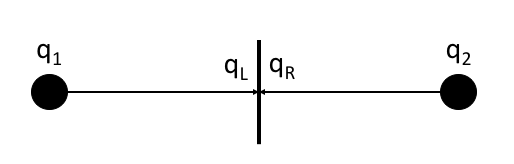
\includegraphics[width=0.5\textwidth]{figures/edge_reconstruction.png}
  \caption{Edge Reconstruction}
  \label{fig:edge-recons}
\end{figure}
%------------------------------------------------------------------------------%
function\cite{van1997comparative}, and varies between 0 and 1 (effectively
blending first-order and second order contributions to the flux evalutation).
The adjoint uses a frozen flux limiter, for purposes that will be discussed in a
later section, and is therefore held as constant in the linearization
computations.  Finally the gradient information $\pd{q_{1,2}}{x}$,
$\pd{q_{1,2}}{y}$, and $\pd{q_{1,2}}{z}$ are computed using least-squares.  For
the example 2-D stencil shown in \fref{fig:lsq-gradients} this is effectively
computed as
%------------------------------------------------------------------------------%
\begin{equation}
  \begin{aligned}
    \pd{q}{x} &= \sum_{i=1}^{5}{W_{x,i}\left( q_i - q_0 \right)} \\
    \pd{q}{y} &= \sum_{i=1}^{5}{W_{y,i}\left( q_i - q_0 \right)} \\
    \pd{q}{z} &= \sum_{i=1}^{5}{W_{z,i}\left( q_i - q_0 \right)}
  \end{aligned}
  \label{grad-construction}
\end{equation}
%------------------------------------------------------------------------------%
where the $z$ direction would come from geometry out of the page.
%------------------------------------------------------------------------------%
\begin{figure}[h]
  \centering
  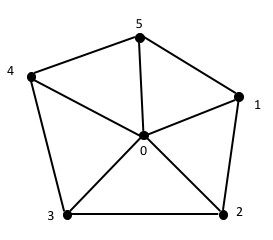
\includegraphics[width=0.5\textwidth]{figures/stencil.png}
  \caption{Example Stencil for Least-Squares Gradient Evaluation}
  \label{fig:lsq-gradients}
\end{figure}
%------------------------------------------------------------------------------%
In practice, the higher order linearizations can be managed easily by
constructing a list of neighboring nodes for each node.  By the chain rule the
linearization of the residual, $R$, is then evaluated in two parts
%------------------------------------------------------------------------------%
\begin{equation}
  \pd{\vR\left(\mq^*\left( \mq \right) \right)}{\mq} = 
  \pd{\vR}{\mq} + \pd{\vR}{\mq^{*}}\pd{\mq^*}{\mq}
  \label{residual-high-low}
\end{equation}
%------------------------------------------------------------------------------%
where $\mq$ are the conserved variables at each node, and $\mq^*$ are the higher
order terms computed in the U-MUSCL reconstruction; therefore, after computing
the exact jacobian of the Roe FDS scheme, $\pd{\vR}{\mq}$, the higher order
linearization is computed by making a circuit around each node to pick up the
contributions from the least squares gradient computation.  For the example
stencil in \fref{fig:lsq-gradients}, the contribution to the residual from
looping around node 0 would be
%------------------------------------------------------------------------------%
\begin{equation}
  \pd{\vR_0}{\mq^*}\pd{\mq^*}{\mq_0} = \pd{\vR_0}{\mq^*} \left[\sum_{i=1}^5{(1-\kappa)
  \left( -W_{x,i}dx - W_{y,i}dy - W_{z,i}dz \right) \pd{q_0}{\mq_0}}\right]
  \label{ho-linearization}
\end{equation}
%------------------------------------------------------------------------------%
An important point that this illustrates is that the linearization of the higher
order terms is not dependent upon the choice of the primitive variable vector
$q$, provided that all of the linearizations are exact.  This is powerful,
because it allows the decoupled scheme to be extended to higher work, without
needing to reformulate the linearizations drastically from the fully-coupled
scheme.
